\chapter{State of the art modelling of comfort}
\label{cha:1}

As discussed in the introduction the goal of the thesis is to learn and implement a method to capture personal experience of comfort in autonomous driving. This will be done by using an inverse optimal control approach where the weights are learned from demonstration. To be able to do this it is necessary that a literature study is done about how to define comfort in a vehicle and to gain information about inverse optimal control.\\
This chapter will give an overview of the literature that is available and will show how the thesis will fit in earlier conducted research.

\section{What are the parameters that define comfort during driving?}
In the following US patent \cite{Daniel2018} the idea is to assess the amount of comfort by calculating a value for carsickness. This value is calculated by a weighted sum of the sway motion, surge motion and heave motion of the vehicle. These motions are being directly calculated from the lateral acceleration, fore-aft acceleration and the vertical acceleration of the vehicle. \\

\begin{figure}[h!]
	\centering
	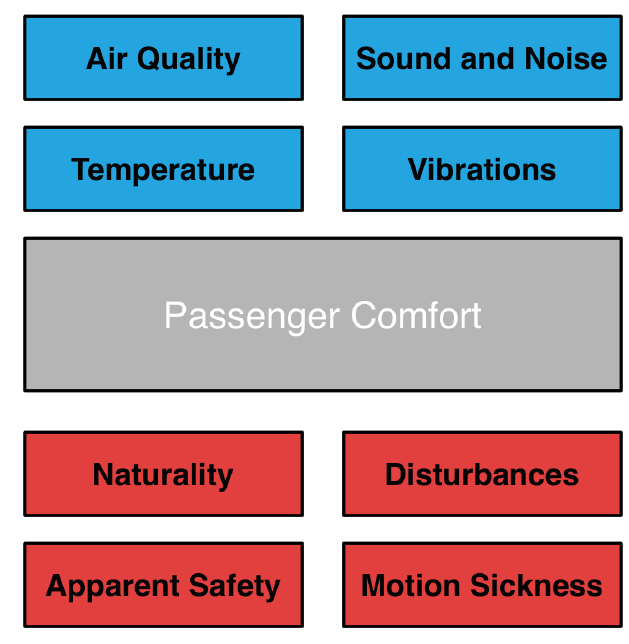
\includegraphics[width=0.48\textwidth]{comfort.PNG}
	\caption{Overview of comfort parameters in autonomous vehicle with old parameters (blue) and new ones (red).(Source: \cite{Elbanhawi2015})}
	\label{fig:Comfort}
\end{figure} 

%\begin{wrapfigure}[22]{L}{0.5\textwidth}
%	\begin{center}
%		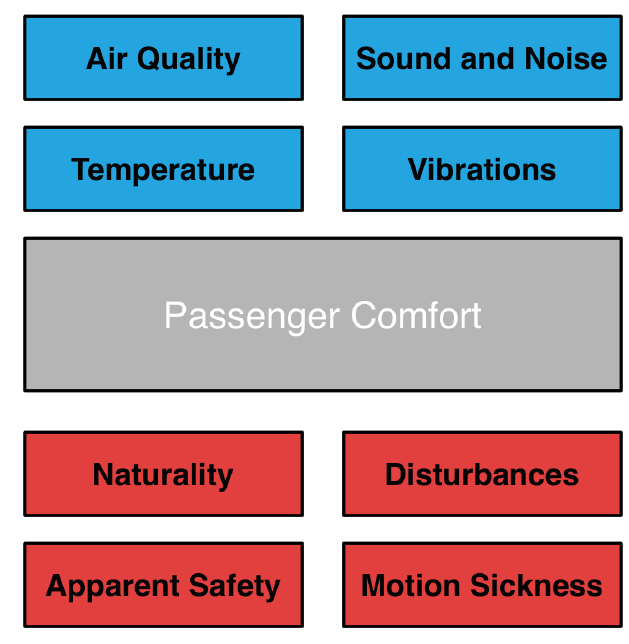
\includegraphics[width=0.48\textwidth]{comfort.PNG}
%	\end{center}
%	\caption{Overview of comfort parameters in autonomous vehicle with old parameters (blue) and new ones (red).(Source: \cite{Elbanhawi2015})}
%	\label{fig:Comfort}
%\end{wrapfigure}
In the paper 'Investigating ride comfort measures in autonomous cars' \cite{Elbanhawi2015}, it is explained that due to the introduction of autonomous vehicles there will be an other perception of comfort. Figure \ref{fig:Comfort} indicates in blue the claimed traditional comfort factors and in red the new ones that also have to be taken into account in when driving in autonomous vehicles. Concretely this can be translated into the preference of smooth trajectories and low lateral motions when the roads are assumed to be sufficiently smooth. A hypotheses is that motion sickness will be more prominent in autonomous driving due to the loss of control. Is is also argued that the amount of travel time and the distance to an obstacle are naturally parameters that contribute to a comfortable feeling. \\

In 'Analysis of Driving Style Preference in Automated Driving' \cite{Bellem} three studies are conducted in order to capture the definition of comfortable driving in autonomous vehicles.
In the first study drivers drove manually with their own driving styles and this data was used in order to look for relevant metrics that could be used in defining distinct driver styles.\\

In a second study the main metrics that were found from study one are varied in order 	 


\subsection{Conclusion}



section{Modelling of comfort}

\subsection{Machine learning}

\subsection{Inverse optimal control}


\subsection{How to model a driver and trajectory}


\subsection{Why do we use the entropy distribution?}


\subsection{RPROP}

\section{Conclusion}

 


















%Dan komt de vraag wat is comfort precies? Literatuur studie...
%Waarnaar kan men kijken als men het over comfort heeft. 
%Lane change bekeken om comfort te valideren --> zeg dat er geen iso standaarden aanwezig zijn.
%Hoe wordt een bestuurder gemoddelleerd --> dit wordt gedaan door een kansverdeling.
%Waarom is entropie nuttig om deze bestuurder te kunnen bekijken? Doe hier meer ondezoek over en verantwoord het gebruik hiervan. Conclusie komt af met comfort parameters die verder worden gebruikt als features.
%Bij de uitleg van de features en waarom er versnelling en acceleratie wordt gebruikt, basseer ook op paper 7 van hoofdpaper
%
%Wat wordt er in de literatuur al gebruikt om comfort te modelleren en geef een overzicht.
%
%Leg uit hoe komt aan entropy distribution komt --> kan beroep doen op ref 2 en 20 van het hoofdrapport (both are assuming an exponential distribution) (IMPORTANT)
%
%Check uitgebreide samenvatting van hoofdpaper op oneNote.
%
%Dit is de reden voor het gebruik van de maximum entropie distributie: 
%	To learn observed behavior, we aim to model the distribution
%	that underlies the empirical sample trajectories.
%	Following Abbeel and Ng [1], we aim to find a model that
%	induces distributions that match, in expectation, the feature
%	values fD of the empirical trajectories D, yielding
%	Ep(x)[f (x)] = fD =
%	1
%	jDj
%	X
%	xk2D
%	f (xk): (1)
%	In general, however, there is not a unique distribution that
%	matches the features. Ziebart et al. [24] resolve this ambiguity
%	by applying the principle of maximum entropy [10], which
%	states that the distribution with the highest entropy represents
%	the given information best since it does not favor any
%	particular outcome besides the observed constraints. (this is the least baised distribution)
%	Modelling expected featueres by hybrid monte carlo method: https://reader.elsevier.com/reader/sd/pii/037026938791197X?token=71567B7640C402F2FF578E34E3BB7914CA14E4A1A29DE88D9534D96C9305E13DA52D0424FF1475A822FCE784725196D3
%%	ref: C:\Users\t2vosx\OneDrive\Documenten\Leuven\Thesis\References2\Citations on main %paper\Learning to Predict Trajectories of Cooperatively Navigating Agents.pdf>
%
% 	paper: Feature-based prediction of trajectories for socially compliant navigation
%	which
%	states that the distribution with the highest entropy represents
%	the given information best since it does not favor any
%	particular outcome besides the observed constraints.
	
%	• Weet dat exponentiële vorm oplossing is van boven staand optimizatie probleem. zie foto
%	--> volgt uit FONC --> oplossing moet (non convex) voldoen aan KKT conditions. Er zijn enkel maar equality constraints aanwezig --> primal feasibility en lagrange stationarity moeten voldaan worden --> LS wordt gecontroleerd drm van de Euler - lagrange vergelijking te gebruiken. 



%\section{The First Topic of the Chapter}
%First comes the introduction to this topic.
%
%
%\subsection{An item}
%Please don't abuse enumerations: short enumerations shouldn't use
%``\verb|itemize|'' or ``\texttt{enumerate}'' environments.
%So \emph{never write}: 
%\begin{quote}
%  The Eiffel tower has three floors:
%  \begin{itemize}
%  \item the first one;
%  \item the second one;
%  \item the third one.
%  \end{itemize}
%\end{quote}
%But write:
%\begin{quote}
%  The Eiffel tower has three floors: the first one, the second one, and the
%  third one.
%\end{quote}
%
%\section{A Second Topic}
%
%
%\subsection{Another item}
%
%
%\section{Conclusion}
%The final section of the chapter gives an overview of the important results
%of this chapter. This implies that the introductory chapter and the
%concluding chapter don't need a conclusion.



%%% Local Variables: 
%%% mode: latex
%%% TeX-master: "thesis"
%%% End: 
